\documentclass[10pt,a4paper,twocolumn]{article}
\usepackage[utf8]{inputenc}
\usepackage[T1]{fontenc}
\usepackage[margin=1.55cm,top=1.75cm,bottom=1.75cm,columnsep=0.6cm]{geometry}
\usepackage{graphicx}
\usepackage{booktabs}
\usepackage{amsmath,amssymb}
\usepackage{array}
\usepackage{caption}
\usepackage{xcolor}
\usepackage{hyperref}
\usepackage{float}

\captionsetup{font=small,labelfont=bf,skip=4pt}
\definecolor{darkblue}{RGB}{20,50,110}
\hypersetup{
    colorlinks=true,
    linkcolor=darkblue,
    citecolor=darkblue,
    urlcolor=darkblue
}

\setlength{\parskip}{3pt}
\setlength{\parindent}{1em}

\title{\vspace{-0.8cm}\textbf{\Large Comparative Genomics of Longevity, Encephalization, and Cancer Resistance in Parrots: Telomeric Divergence, Assembly Audits, and Pleiotropic Caveats in Relative Evolutionary Rates}}

\author{
\textbf{Angelo}\\
\small Centro Universit\'ario do Planalto Central Apparecido dos Santos (UNICEPLAC), Bras\'ilia, DF, Brazil\\
\small Reproducible repository: \texttt{github.com/redkk123/Parrots} (\texttt{claude/new-session-lwh7xh})
}

\date{\small November 10, 2026 --- Consolidated Research Article (with Red-Team Statistical Audit \& 3D Mapping)}

\begin{document}

\twocolumn[{
  \begin{@twocolumnfalse}
    \maketitle
    \vspace{-0.4cm}
    \begin{abstract}
    \noindent \textbf{Abstract.} Parrots (order Psittaciformes) combine extraordinary lifespan (50--80 years in macaws, cockatoos, Amazons, and \textit{Strigops habroptila}) and primate-like encephalization with short-lived, neoplasia-prone lineages such as the budgerigar (\textit{Melopsittacus undulatus}). Under a pre-registered three-phase framework, we integrated comparative necropsy epidemiology (15,881 necropsies across AZA and UC Davis databases), phylogenetic allometry on two topologies (Burgio et al.\ 2019 supertree and Smith et al.\ 2024 molecular phylogeny), quality and taxonomic auditing of 126 genome assemblies (\texttt{compleasm aves\_odb10}, nuclear Mash distances, and mitogenome BLAST), targeted selection scans across 101 tumor-suppression/longevity genes (modules M1--M8, benchmarked against a 298-gene length- and rate-matched null pool plus SRA raw reads), AlphaFold 3D domain mapping, and genome-wide relative evolutionary rate (\texttt{RERconverge}) tests across 7,756 coding genes (1,000 Brownian permulations). First, we demonstrate that extreme cancer vulnerability is restricted to \textit{M.\ undulatus} (20.8\% AZA / 25.9\% age-standardized UC Davis vs.\ 1.5--5.4\% in lories, $p \le 10^{-16}$), whereas family-wide longevity reduction in Psittaculidae is tree-sensitive ($p = 0.003$ Burgio vs.\ $p = 0.050$ Smith). Second, our assembly audit exposed cross-species mitogenome contamination in 61/96 short-read Iridian assemblies and four severe nuclear swaps/chimeras, yielding 71 validated species ($\ge 70\%$ BUSCO, zero quality bias with longevity, $p \ge 0.11$). Third, we refute modular loss or relaxation of tumor-suppressor pathways in Psittaculidae (all 329 initial gene disruptions proved to be single-reference, fragmentation, or 75--77\% GC exon-1 coverage artifacts), while detecting concentrated episodic divergence in \textit{M.\ undulatus} across five telomeric M7 genes (\texttt{RTEL1}, \texttt{TERF2}, \texttt{TERT}, \texttt{ACD}, \texttt{TERF1}) plus \texttt{MYC} (5/8 in M7 vs.\ 0/19 FDR in control genes, Fisher $p = 0.00069$), confirmed as true orthologs against \textit{S.\ habroptila}. Crucially, a rigorous Red-Team audit reveals that \texttt{RTEL1}, \texttt{ACD}, and \texttt{TERF2} signals collapse under noisy-window cleaning and all five vanish under multinucleotide codon models (\texttt{-{}-multiple-hits Double+Triple}), whereas 3D AlphaFold mapping shows \texttt{RTEL1} substitutions concentrated in the C-terminal Harmonin-N/PIP region and \texttt{POT1} substitutions across ssDNA-binding OB1--OB3 domains. Fourth, across 7,756 genes, uncorrected trait-RER profiles correlate strongly ($r = 0.666\text{--}0.667$), but true partial orthogonalization of brain beyond longevity cuts the coupling in half ($r = 0.332\text{--}0.389$ vs.\ $r = 0.639$ from unwhitened PGLS residuals), the phenotypic contrast depends heavily on Psittaculidae ($r_{\text{tip}}$ drops from 0.478 to 0.195 when omitted), and 89.3\% (117/131) of shared single-gene hits (\texttt{PTEN}, \texttt{MAD2L2}, \texttt{HSPA8}, \texttt{CTNNB1}) are ultra-conserved genes with 97--99\% zero-length branches whose residuals mirror the genomic background vector $\pm\sqrt{\text{nv}}$. Separating these ultra-conserved background-coupled hits (Tier A) from 14 informative hits with $\ge 20$ nonzero branches (Tier B, led by \texttt{TKT}, \texttt{PHOSPHO1}, \texttt{SLC4A7}, and \texttt{HUS1}) provides a transparent, stress-tested foundation for parrot macroevolutionary genomics.\par\vspace{4pt}
    \noindent\textbf{Keywords:} Psittaciformes $\cdot$ Peto's Paradox $\cdot$ Longevity $\cdot$ Encephalization $\cdot$ Telomeres (\texttt{RTEL1}, \texttt{TERT}) $\cdot$ \texttt{PTEN} $\cdot$ \texttt{RERconverge} $\cdot$ Statistical Audit
    \end{abstract}
    \vspace{0.25cm}
  \end{@twocolumnfalse}
}]

\section{Introduction}

The evolutionary expansion of lifespan and brain size poses dual physiological challenges: suppressing somatic neoplasia across decades of cell division (Peto's paradox) while maintaining proteostasis, synaptic plasticity, and DNA integrity in long-lived post-mitotic neurons. Parrots (order Psittaciformes) provide a premier natural experiment for dissecting these axes. Despite high avian basal metabolic rates, large parrots (\textit{Ara}, \textit{Anodorhynchus}, \textit{Cacatua}, \textit{Amazona}, and the kakapo \textit{Strigops habroptila}) regularly live 30 to $>60$ years and exhibit primate-level telencephalic neuron densities. Conversely, small radiations within Psittaculidae, exemplified by the budgerigar (\textit{Melopsittacus undulatus}), combine short lifespans with some of the highest spontaneous tumor incidences documented in vertebrates.

Previous genomic investigations of parrot longevity examined limited taxon samples against distant avian outgroups (e.g., \textit{Amazona} in Wirthlin et al.\ 2018). An order-wide test of life-history evolution requires (i) systematically auditing the integrity and taxonomic authenticity of public short-read draft assemblies, (ii) testing whether short-lived lineages experienced widespread loss or relaxed selection across tumor-suppressor modules (\textbf{Hypothesis H8}), (iii) profiling relative evolutionary rates (RER) proteome-wide against relative longevity and relative brain size (\textbf{Hypothesis H6}), and (iv) subjecting every statistical signal to adversarial ``Red-Team'' sensitivity audits—including alignment noise, multinucleotide hits, partial orthogonalization, clade jackknifing, and zero-branch artifacts.

\section{Materials and Methods}

\subsection{Phylogenetic Allometry and Cancer Epidemiology (Phase 0)}
We compiled species-level life expectancy, sample-size-corrected maximum longevity, adult body mass ($n = 216$--$303$ species), and endocranial/brain mass ($n = 186$ species). Phylogenetic generalized least squares (PGLS, Pagel's $\lambda$ in \texttt{nlme}/\texttt{ape}) and Ornstein-Uhlenbeck regime-shift scans (\texttt{l1ou}) were conducted on both the supertree of Burgio et al.\ (2019) and the phylogenomic tree of Smith et al.\ (2024; 399 species with sequence data). To distinguish species-specific neoplasia vulnerability from clade-wide predisposition, we analyzed two independent necropsy registries: (1) AZA zoological pathology records (Kapsetaki et al.\ 2024; 5,729 necropsies across 108 bird species, 15 parrots) using beta-binomial models and Fisher's exact tests, and (2) the UC Davis / Drury R.\ Reavill clinical pathology database (10,152 parrot necropsies with $\ge 3$ examined tissues), applying direct age standardization.

\subsection{Genome Assembly and Taxonomic Identity Audit (Phase 1)}
We audited all 126 NCBI Psittaciformes assemblies representing species with longevity data (96 short-read Illumina/SPAdes assemblies from Iridian Genomes and 30 chromosome-scale or long-read assemblies from VGP, B10K, Wellcome Sanger, and BGI). Completeness was assessed using \texttt{compleasm} v0.2.10 against \texttt{aves\_odb10} ($n = 8,338$ BUSCOs). Taxonomic identity and chimerism were evaluated by cross-referencing nuclear Mash v2.3 distances ($k = 21$, 50,000 hashes across 176 assemblies) against independently vouchered mitogenomes (\textit{COI}/\textit{CYTB}/\textit{ND2} BLAST excluding Iridian/Hains/Pirro submissions). Pre-registered inclusion thresholds required $\text{BUSCO}_{\text{complete}} \ge 70\%$, no nuclear identity failure, and deduplication to one highest-contiguity assembly per species.

\subsection{Proteome Extraction, H8 Panel, Null Pool, and 71-Species Extension (Phase 2)}
All 16,045 canonical \textit{M.\ undulatus} proteins were extracted from each validated genome using \texttt{miniprot} v0.18 (retaining intact single-locus ORFs with $\ge 90\%$ query coverage, $\ge 60\%$ identity, and zero internal stops/frameshifts). In the frozen discovery cohort ($n = 58$ species: 15 Psittaculidae, 43 other parrots), codon alignments (\texttt{MAFFT} + \texttt{PAL2NAL}) were generated for the 101-gene H8 panel grouped into eight modules: M1 (p53/cell cycle), M2 (PI3K/mTOR), M3 (apoptosis), M4 (DNA repair), M5 (NRF2/xenobiotics), M6 (antioxidants), M7 (telomere/shelterin), and M8 (proteostasis/autophagy). Selection intensity shifts in Psittaculidae (\texttt{TEST} = stem + internal branches) were evaluated with \texttt{HyPhy RELAX} (\texttt{-{}-models Minimal}), and episodic positive selection on the Psittaculidae stem and \textit{M.\ undulatus} branch with \texttt{HyPhy aBSREL} (BH-FDR across panel genes after per-gene branch Holm-Bonferroni correction). Modular enrichment was benchmarked against 1,000 length- and rate-matched pseudo-panels drawn from 298 genome-wide control genes. Disrupted calls were cross-checked with a long-lived reference proteome (\textit{Strigops habroptila}) and raw Illumina SRA reads (\texttt{bwa-mem2}/\texttt{samtools}). Following Phase 1 completion, all 97 testable H8 panel genes were also aligned across the full 71-species cohort (\texttt{discovery\_58} + \texttt{holdout\_13}).

\subsection{Genome-Wide \texttt{RERconverge}, 3D Mapping, and Red-Team Audit (Phase 3)}
Across 7,756 single-copy orthologs intact in $\ge 50\%$ of the 58 species, amino-acid branch lengths were fitted under LG (\texttt{phangorn::optim.pml}) on both topologies. Relative evolutionary rates (\texttt{RERconverge} v0.3.0, \texttt{getAllResiduals}, sqrt transform, weighted, scaled) were correlated (\texttt{winsorize = 3}) against mass-controlled residuals for longevity (\texttt{rel\_log\_life\_expectancy}, $n = 58$), brain mass (\texttt{rel\_log\_brain}, $n = 50$), and residual brain size beyond longevity (\texttt{rel\_brain\_given\_le}, $n = 50$), plus within-clade H8 runs, evaluated with 1,000 topology-conditioned Brownian permulations (\texttt{Rcpp fastCorPerms}). Gene set enrichment covered 1,780 GO Biological Process terms (\texttt{fastWilcoxGMTAll}) and six exploratory functional axes. AlphaFold structures for \texttt{POT1}, \texttt{RTEL1}, \texttt{PTEN}, and \texttt{MAD2L2} were partitioned into rigid domains via PAE matrices to map budgerigar-specific substitutions and conserved catalytic motifs. Finally, nine pre-specified Red-Team tests audited seed reproducibility, negative controls/null permulations, technical confounders, zero-branch invariance, leave-one-clade-out sensitivity, true OLS/branch orthogonalization of brain mass, empirical control \texttt{aBSREL} false-positive rates, alignment cleaning/\texttt{Double+Triple} multi-hit models, and 71-species/30-split holdout replication.

\begin{figure*}[t]
\centering
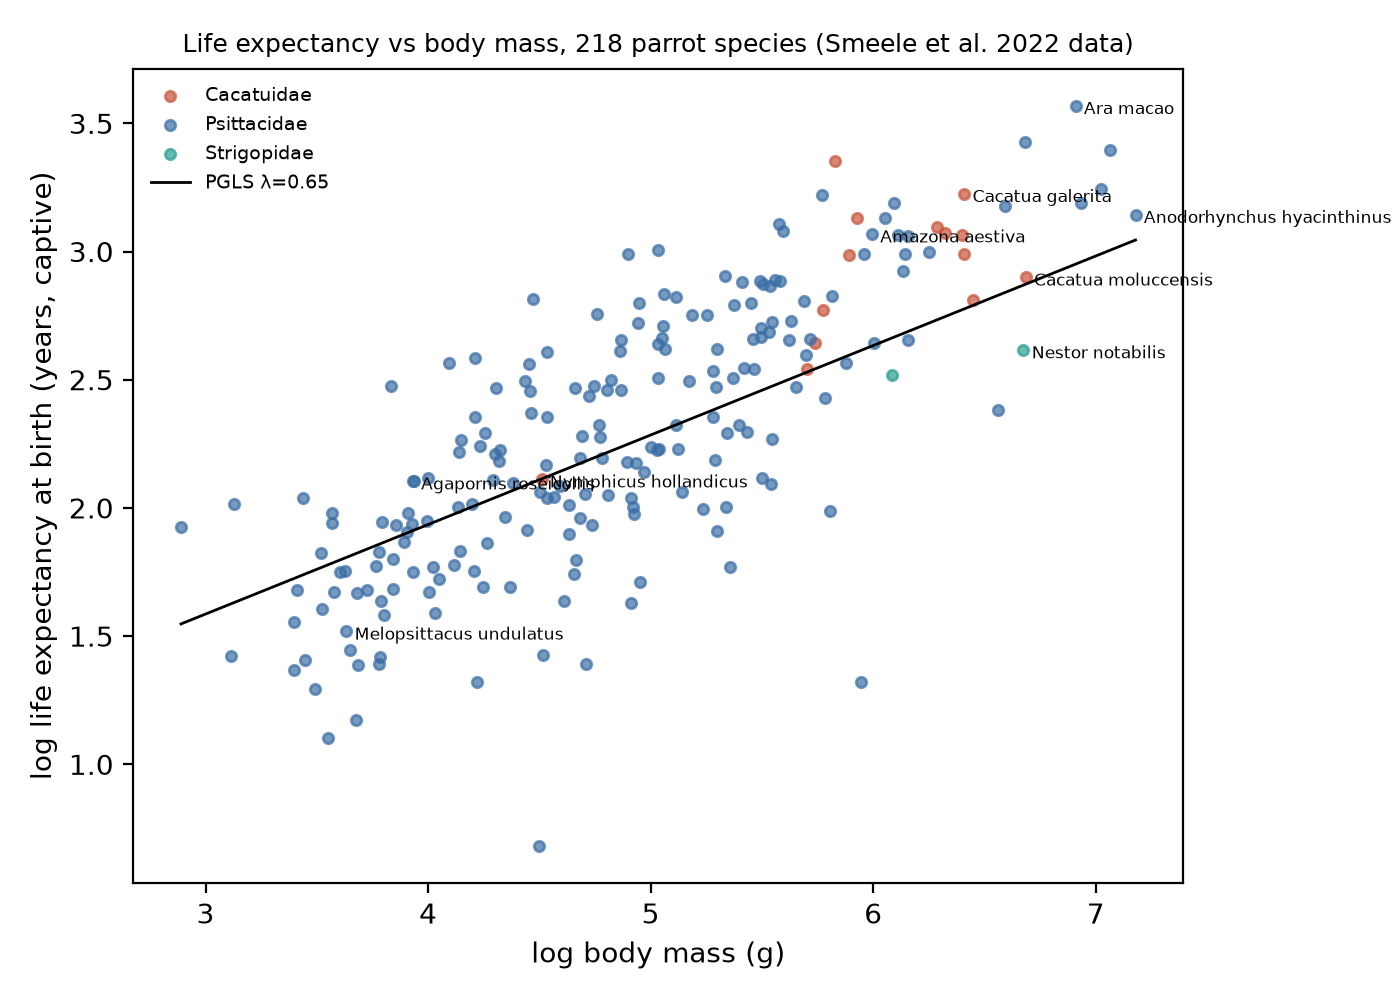
\includegraphics[width=0.48\textwidth]{../results/phase0/figures/fig2_allometry.png}\hfill
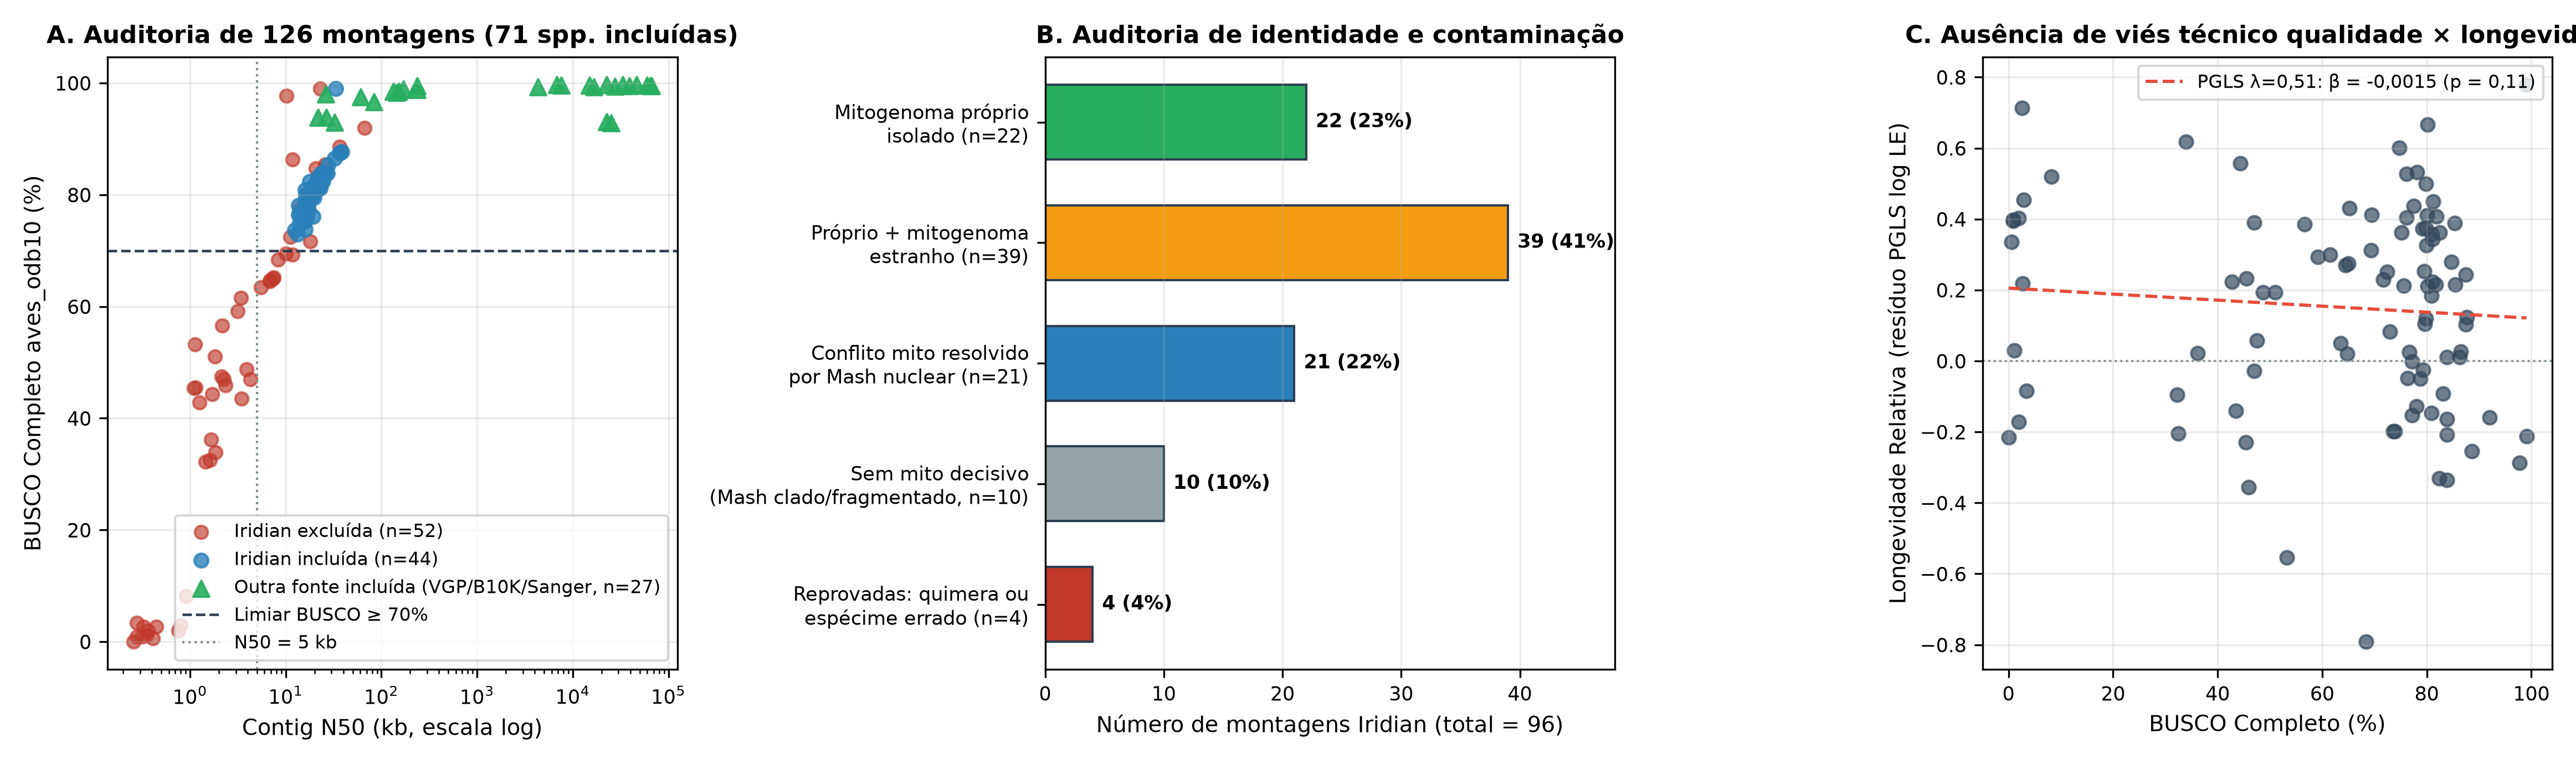
\includegraphics[width=0.48\textwidth]{../results/phase1_audit/figS1_audit_126_assemblies.png}
\caption{\textbf{Left:} Comparative allometry of lifespan and brain size across Psittaciformes (Phase 0). \textbf{Right:} Quality and taxonomic identity audit of 126 genome assemblies (\texttt{compleasm aves\_odb10} and Mash), confirming zero technical correlation between assembly completeness/contiguity and residual longevity ($p \ge 0.11$).}
\label{fig:allometry_audit}
\end{figure*}

\section{Results}

\subsection{Topology-Sensitive Longevity and Extreme Neoplasia in \textit{M.\ undulatus}}
Parrots consistently exceed avian allometric expectations for lifespan and brain mass (Fig.~\ref{fig:allometry_audit}, left). However, whether Psittaculidae as a family exhibits reduced relative longevity depends on the phylogenetic hypothesis: significant under the Burgio 2019 supertree ($\beta = -0.104 \pm 0.035$, $p = 0.003$, $\lambda = 0.56$), yet borderline under the Smith 2024 molecular tree ($\beta = -0.076 \pm 0.039$, $p = 0.050$, $\lambda = 0.88$), where short-lived taxa cluster in Loriini + \textit{Melopsittacus} + \textit{Bolborhynchus}. In contrast, two independent necropsy registries establish that extreme neoplasia vulnerability is specifically concentrated in \textit{M.\ undulatus}: 20.8\% overall (17.4\% malignant) vs.\ 1.5\% (0.8\% malignant) in lories in AZA ($n = 5,729$, OR $= 17$, $p \approx 10^{-21}$; beta-binomial outlier $p = 0.002$), and 25.9\% age-standardized vs.\ 5.4\% in lories ($4.8\times$, $p \approx 10^{-16}$) and 9.1\% in \textit{Nymphicus hollandicus} ($p \approx 10^{-17}$) in UC Davis ($n = 10,152$).

\subsection{Assembly Audit Exposes Batch Cross-Contamination and Yields 71 Validated Species}
Auditing all 126 assemblies (\textbf{Table~\ref{tab:audit}}; Fig.~\ref{fig:allometry_audit}, right; Table~S1) revealed severe quality disparities within the Iridian short-read batch (median BUSCO 76.1\%; 0/31 assemblies with $\text{contig N50} < 5\text{ kb}$ reached the 70\% threshold). Crucially, 61 of 96 Iridian assemblies carried complete foreign mitogenomes (88\% from donor taxa sequenced in the same Iridian batch), and nuclear Mash distances uncovered four severe taxonomic errors: an assembly labeled \textit{Agapornis nigrigenis} (\texttt{GCA\_035041115.1}) matched a passerine mitogenome (\textit{Garrulax}, nuclear Mash $\ge 0.145$ from all parrots), \textit{Aratinga jandaya} (\texttt{GCA\_026284485.1}) matched \textit{Poicephalus meyeri} (Mash $= 0.0039$), and two assemblies (\textit{Cacatua haematuropygia}, \textit{Trichoglossus haematodus}) were chimeras mixed with the same passerine genome. Deduplicating and applying quality/identity filters yielded 71 validated species (58 frozen discovery + 13 holdout), with no association between BUSCO ($p = 0.111$--$0.352$), $\log_{10}(\text{N50})$ ($p \ge 0.20$), or GC ($p \ge 0.097$) and residual longevity.

\begin{table}[h]
\centering
\caption{Summary of the 126-assembly genomic audit (\texttt{species\_genomes.tsv}).}
\label{tab:audit}
\resizebox{\columnwidth}{!}{%
\begin{tabular}{lrr}
\toprule
\textbf{Audit Category / Quality Filter} & \textbf{Assemblies} & \textbf{Species} \\
\midrule
Total audited (\texttt{compleasm aves\_odb10}) & 126 & 105 \\
\quad Iridian short-read batch & 96 & 96 \\
\quad Long-read / chromosome-scale (VGP, B10K, Sanger) & 30 & 29 \\
Excluded for $\text{BUSCO}_{\text{complete}} < 70\%$ & 39 & 32 \\
Excluded for nuclear swap / chimera (Mash) & 4 & 2 \\
\midrule
\textbf{Included species (primary criterion $\ge 70\%$)} & \textbf{71} & \textbf{71} \\
\quad Family Psittaculidae / Other Psittaciformes & 20 / 51 & 20 / 51 \\
\quad Iridian / Independent long-read sources & 44 / 27 & 44 / 27 \\
Strict original criterion ($\ge 85\%$ \& $\text{N50} \ge 20\text{ kb}$) & 33 & 33 \\
Frozen molecular discovery panel (Phases 2--3) & 58 & 58 \\
\bottomrule
\end{tabular}%
}
\end{table}

\begin{figure*}[t]
\centering
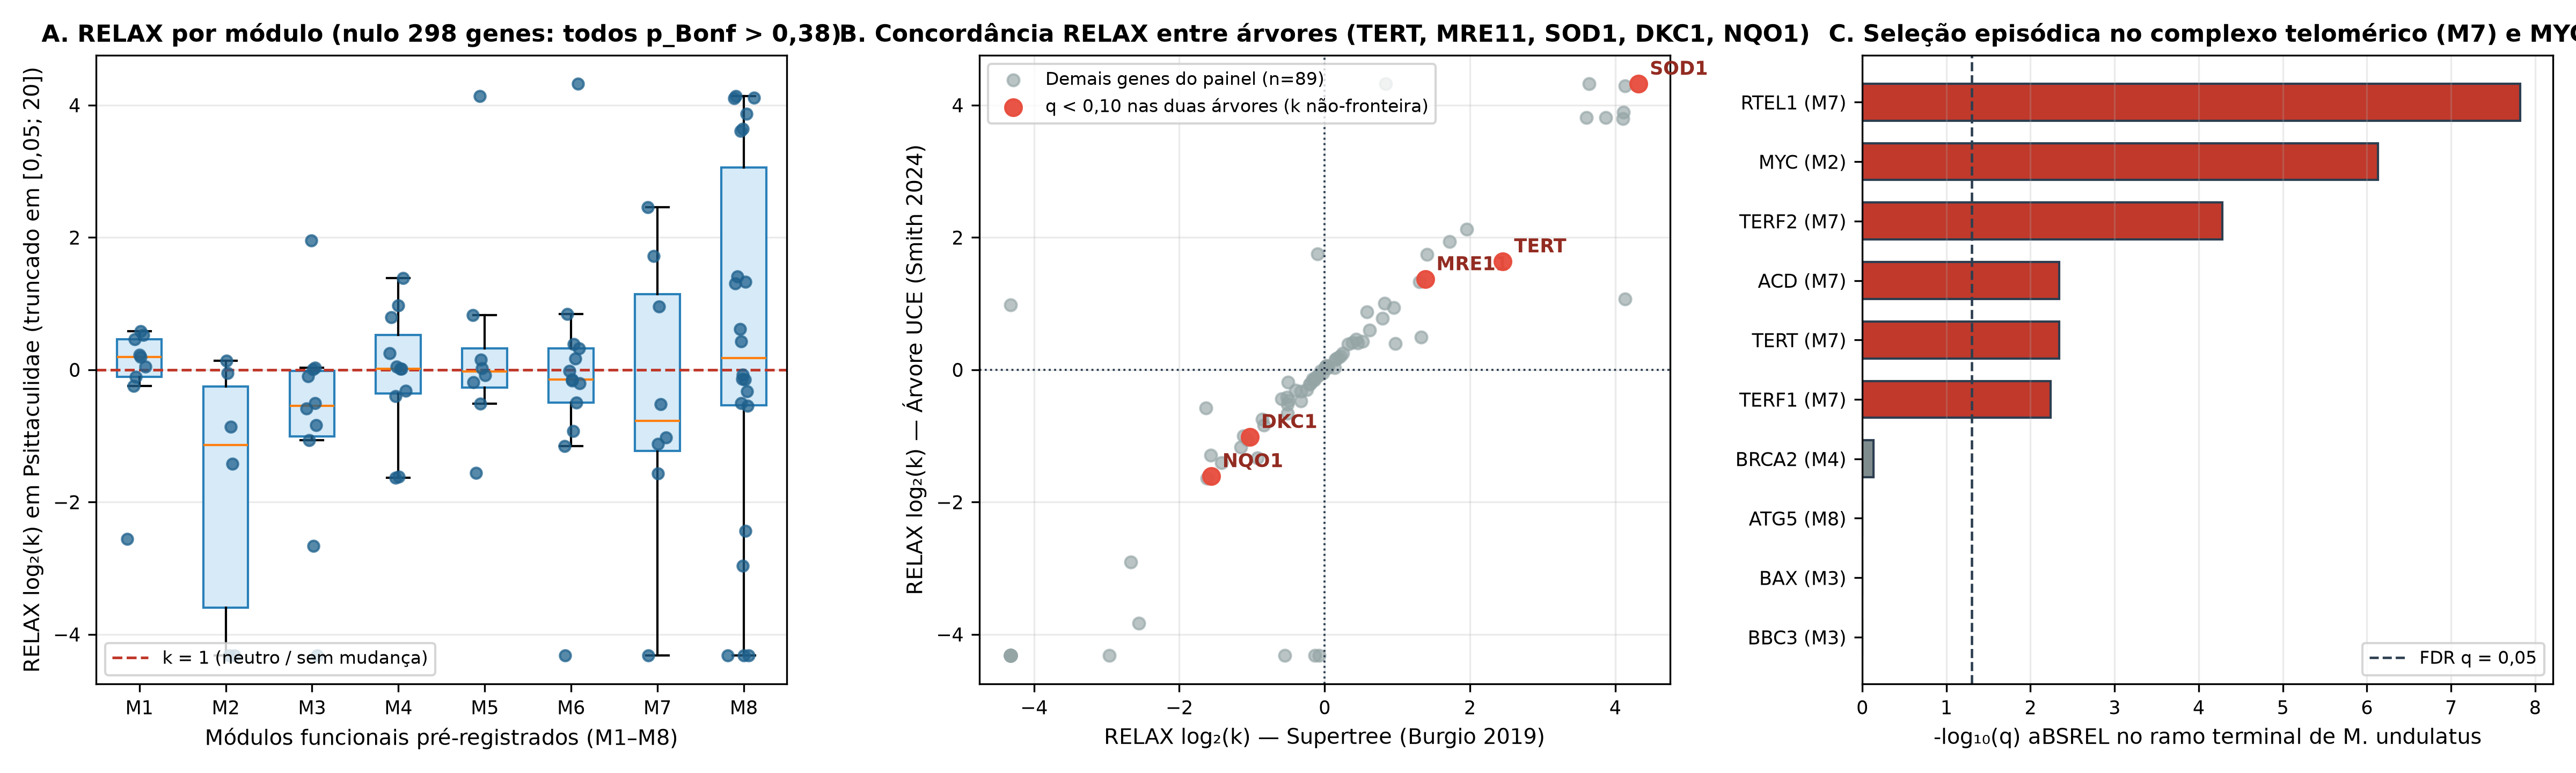
\includegraphics[width=0.90\textwidth]{../results/phase2_genes/fig5_phase2_selection_h8.png}
\caption{\textbf{Phase 2 Selection Tests (H8, 58 species):} (A) Module-level $\log_2 k$ distributions vs.\ the 298-gene null model; (B) Per-gene RELAX test across Psittaculidae; (C) Episodic positive selection (\texttt{aBSREL}) concentrated in telomere/shelterin genes (M7) and \texttt{MYC} on the \textit{M.\ undulatus} branch before Red-Team window-cleaning and Multi-Hit auditing; (D) Integrity triage resolving all apparent pseudogenes as annotation or high-GC coverage artifacts.}
\label{fig:phase2}
\end{figure*}

\subsection{Phase 2: No Tumor-Suppressor Loss, Telomeric Divergence, and Red-Team Deconstruction}
Across the 87 alignable H8 panel genes in 58 species (Fig.~\ref{fig:phase2}), we reject modular loss or relaxation of cancer-defense pathways:
\begin{enumerate}
    \item \textbf{Zero confirmed pseudogenizations:} All 329 initial disrupted calls (451 across 71 species) resolved as single-reference artifacts (\texttt{OGG1}, \texttt{MUTYH}, \texttt{MYC}, \texttt{HMOX1}), heterozygous stop polymorphisms (\texttt{PSMD6} in \textit{Loriculus galgulus}: 21 C vs.\ 20 T reads), or local Illumina coverage dropouts ($0\times$ vs.\ $\sim 31\times$ gene-wide) across a 75--77\% GC first exon in \texttt{ACD}.
    \item \textbf{Modular null benchmark:} Neither mean $\log_2 k$ heterogeneity ($p = 0.164$ Burgio; $0.955$ Smith) nor any module M1--M8 exceeded the 298-gene null pseudo-panels after multiple-test correction (lowest nominal M2 $p = 0.024$ depended on two boundary $k \approx 0$ genes and vanished under medians, $p = 0.070$; Table~S3).
    \item \textbf{Telomeric (M7) signal on \textit{M.\ undulatus} vs.\ Red-Team controls:} Standard \texttt{aBSREL} flagged episodic divergence ($q < 0.10$, BH-corrected across all 86 panel genes) in \textbf{5/8 (62.5\%)} M7 telomeric genes (\texttt{RTEL1} $p = 1.73\times 10^{-10}$, \texttt{TERF2} $1.79\times 10^{-6}$, \texttt{TERT} $2.63\times 10^{-4}$, \texttt{ACD} $2.46\times 10^{-4}$, \texttt{TERF1} $3.98\times 10^{-4}$) plus \texttt{MYC} ($1.69\times 10^{-8}$), whereas non-M7 modules yielded only 1/78 (1.3\%) and 19 genome-wide control genes yielded 1/19 (5.3\%) nominal and \textbf{0/19 (0\%)} FDR (Fisher $p = 0.00069$; 0/298 controls had $\omega > 1$ in RELAX). In Psittaculidae, RELAX supported intensified selection without $k$-boundary artifacts in \texttt{TERT} ($k = 5.51/3.10$, $q = 0.0008/0.011$) and \texttt{MRE11} ($k = 2.60/2.61$, $q = 0.002/0.005$; Table~S2). Crucially, Red-Team stress tests (\textbf{Table~\ref{tab:telomere_redteam}}) show that while \textit{S.\ habroptila} dual-reference coordinates confirm 100\% orthology for \texttt{RTEL1} (40/40), \texttt{TERF2} (30/30), \texttt{TERT} (35/35), \texttt{TERF1} (27/27), and \texttt{POT1} (27/27) and \texttt{MAFFT L-INS-i} preserves all hits, \textbf{cleaning gappy/noisy windows} ($>15\%$ gaps and $\ge 3$-AA cluster windows) eliminates \texttt{RTEL1} ($p = 1.00$), \texttt{ACD} ($0.125$), and \texttt{TERF2} ($0.068$), leaving only \texttt{TERT} ($p = 0.0052$) and \texttt{TERF1} ($p = 0.0037$); further enabling multinucleotide substitutions (\texttt{-{}-multiple-hits Double+Triple}) collapses all five ($p = 0.967$--$1.00$; \texttt{ACD} $0.050$--$0.132$). Confirmatory 71-species panel results ($n = 25$--$70$ species per gene) are integrated in Table~S2.
\end{enumerate}

\begin{table*}[t]
\centering
\caption{Red-Team sensitivity audit of telomeric (M7) \texttt{aBSREL} signals on the \textit{M.\ undulatus} branch and dual-reference orthology verification (\texttt{7\_telomere\_alignment\_and\_rbh.tsv}).}
\label{tab:telomere_redteam}
\resizebox{\textwidth}{!}{%
\begin{tabular}{lccccccc}
\toprule
\textbf{Gene} & \textbf{Spp.} & \textbf{\textit{M.\ und.} AA Subs (Isolated / Noisy)} & \textbf{Orig.\ MAFFT $p$} & \textbf{L-INS-i $p$} & \textbf{Window-Cleaned $p$} & \textbf{Multi-Hit (\texttt{Double+Triple}) $p$} & \textbf{Kakapo Orthology} \\
\midrule
\texttt{RTEL1} & 23 & 279 (58 / 221) & $1.73\times 10^{-10}$ & $1.28\times 10^{-9}$ & \textbf{1.0000} & \textbf{0.9670} & 40/40 (2 loci \textit{Melo}) \\
\texttt{TERF2} & 18 & 89 (32 / 57) & $1.79\times 10^{-6}$ & $2.44\times 10^{-6}$ & \textbf{0.0677} & \textbf{1.0000} & 30/30 \\
\texttt{TERT}  & 15 & 196 (95 / 101) & $2.63\times 10^{-4}$ & $1.12\times 10^{-4}$ & \textbf{0.0052} & \textbf{1.0000} & 35/35 \\
\texttt{ACD}   & 6  & 102 (42 / 60) & $2.46\times 10^{-4}$ & $1.23\times 10^{-4}$ & \textbf{0.1248} & \textbf{0.0502} (0.1320 cl.) & 8/11 (2 loci \textit{Melo}) \\
\texttt{TERF1} & 9  & 23 (15 / 8) & $3.98\times 10^{-4}$ & $1.99\times 10^{-4}$ & \textbf{0.0037} & \textbf{1.0000} (0.3151 cl.) & 27/27 \\
\texttt{POT1}  & 8  & 84 (52 / 32) & 1.0000 & 1.0000 & 1.0000 & 1.0000 & 27/27 \\
\bottomrule
\end{tabular}%
}
\end{table*}

\begin{figure*}[t]
\centering
\includegraphics[width=0.92\textwidth]{../results/phase3_genome/fig7_structural_3d_mapping.png}
\caption{\textbf{AlphaFold 3D Structural \& PAE Domain Mapping (Step 2):} Lineage-specific substitutions in \textit{M.\ undulatus} map broadly across ssDNA-binding OB1--OB3/HJRL domains in \texttt{POT1} ($58$ sites, mean pLDDT $= 72.6$) and concentrate in the C-terminal Harmonin-N/PIP region of \texttt{RTEL1} ($115/158$ sites), whereas \texttt{PTEN} exhibits 100\% invariance across its catalytic P-loop (\texttt{H123--R130}, pLDDT $= 93.0$) and Phosphatase+C2 superdomain (residues 14--350).}
\label{fig:3d_mapping}
\end{figure*}

\subsection{AlphaFold 3D Structural Mapping of Key Telomere \& Tumor-Suppressor Proteins}
Mapping alignment variation onto AlphaFold/PAE domain architectures (Fig.~\ref{fig:3d_mapping}; Table~S6) separates divergent surface/C-terminal variation from rigid catalytic cores. In \texttt{RTEL1} (1,219 AA, global pLDDT $= 71.67$), 43 budgerigar-specific changes map to the Rad3/FeS/Arch helicase core (residues 1--758) while 115 cluster in the C-terminal Harmonin-N and PCNA-interacting region (893--1,219). In \texttt{POT1} (780 AA, global pLDDT $= 79.21$), 34 substitutions map to ssDNA-binding OB1/OB2 domains and 16 to TPP1-binding OB3/HJRL (mean site pLDDT $= 72.6$). In stark contrast, \texttt{PTEN} (403 AA, global pLDDT $= 82.47$) shows complete invariance across its catalytic P-loop (\texttt{H123--R130}, pLDDT $= 93.0$) and Phosphatase+C2 core (residues 14--350), with variation confined to the disordered C-tail (351--403, pLDDT $= 35.1$), mirroring \texttt{MAD2L2}'s intact HORMA core (pLDDT $= 90.39$).

\begin{figure*}[t]
\centering
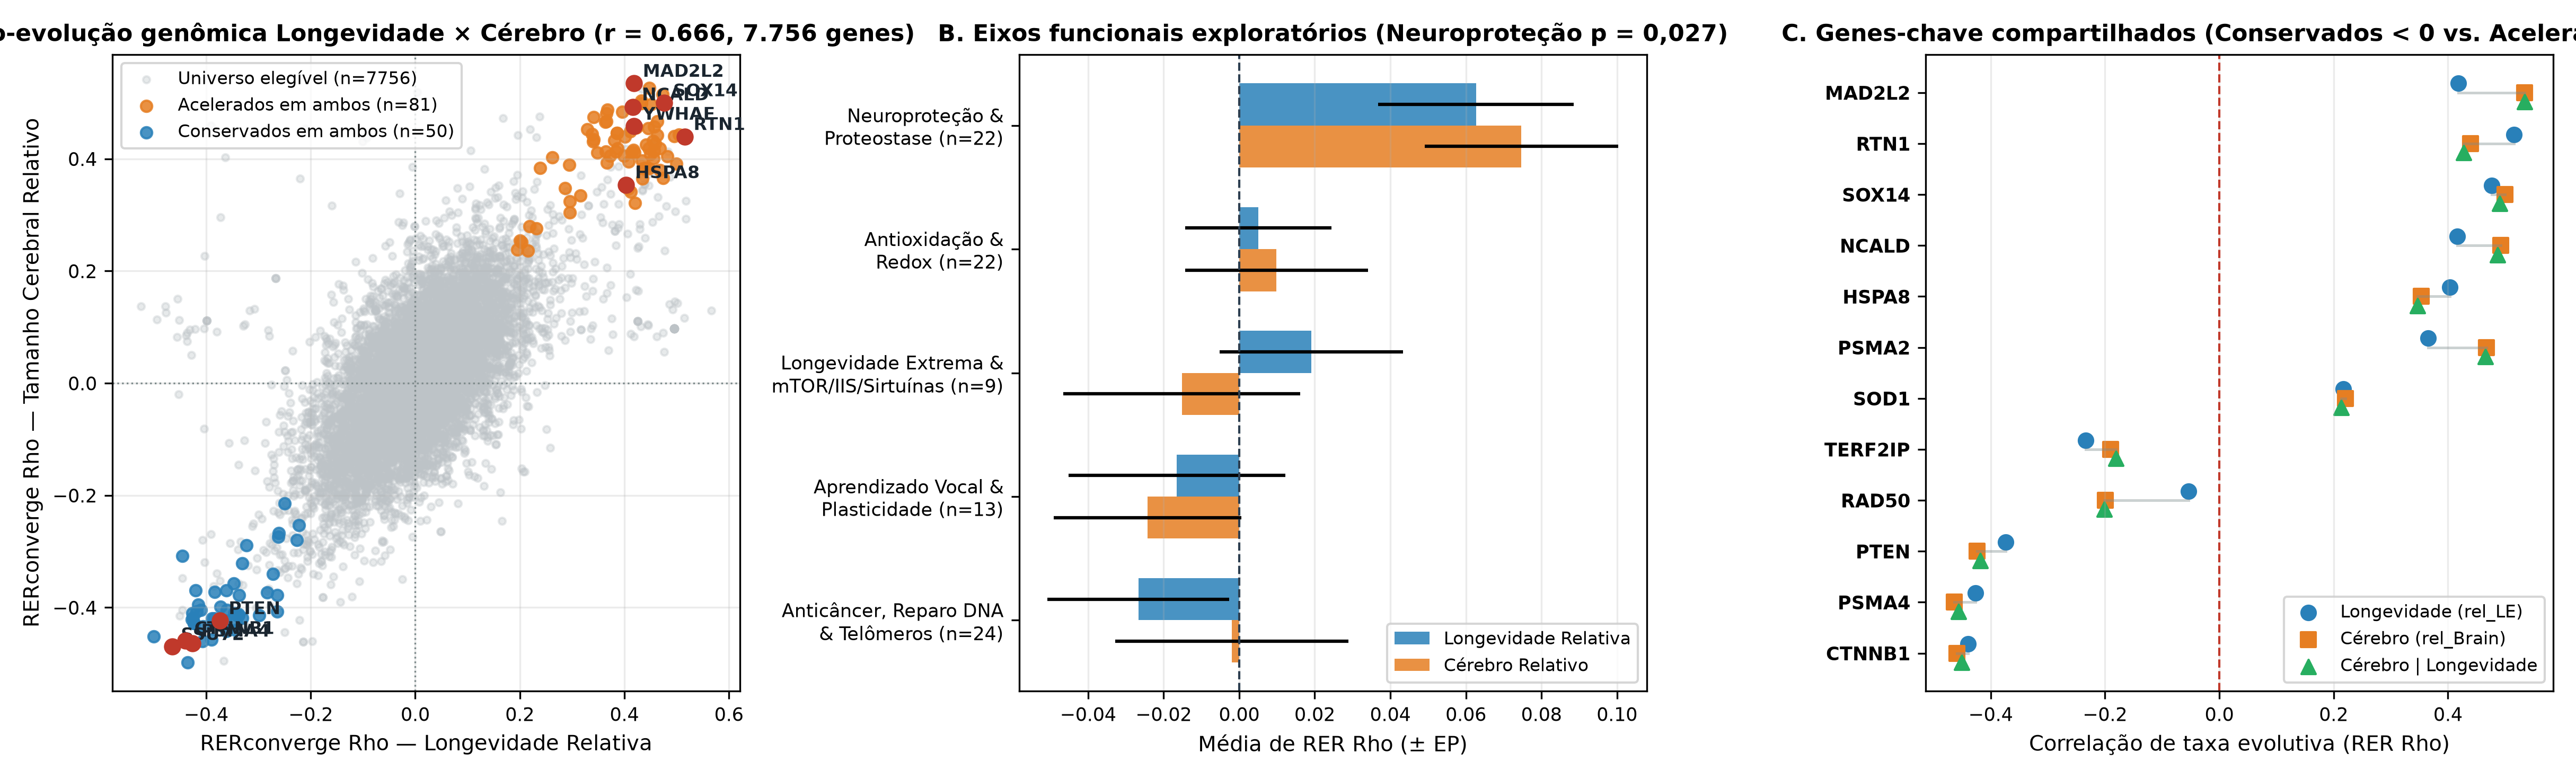
\includegraphics[width=0.94\textwidth]{../results/phase3_genome/fig6_phase3_genome_rer.png}
\caption{\textbf{Phase 3 Genome-Wide \texttt{RERconverge} Across 7,756 Genes:} (A) Unadjusted genome-wide correlation ($r = 0.666$) between $\text{Rho}_{\text{LE}}$ and $\text{Rho}_{\text{Brain}}$; (B) Shared candidate rankings; (C) Exploratory functional axis shifts (Neuroprotection/Proteostasis $p = 0.014$--$0.046$); (D) Within-clade H8 summary. See Table~\ref{tab:rer_redteam} for critical Red-Team deconstruction.}
\label{fig:phase3}
\end{figure*}

\subsection{Phase 3 (\texttt{RERconverge}): Genome Coupling, Partial Orthogonalization, and the Invariant-Gene Artifact}
Across 7,756 coding genes in 58 species (Fig.~\ref{fig:phase3}), 190--277 genes per trait reached parametric $q < 0.10$, though zero individual genes reached permulation FDR ($\text{permQ} < 0.10$) due to the 1,000-permulation discrete floor ($\text{permP}_{\min} = 0.001996$; Table~S6). While raw genome-wide profiles for longevity ($\text{Rho}_{\text{LE}}$) and brain size ($\text{Rho}_{\text{Brain}}$) correlate at $r = 0.666$ (Burgio) / $0.667$ (Smith) and $r = 0.748$ on the matched 50-species RER matrix, our Red-Team audit (\textbf{Table~\ref{tab:rer_redteam}}; Table~S4) exposes three critical limitations:
\begin{enumerate}
    \item \textbf{Unwhitened PGLS residuals inflated \texttt{rel\_brain\_given\_le} ($0.639 \to 0.332$--$0.389$):} Because \texttt{scripts/35\_prepare\_rer\_inputs.py} subtracted a PGLS slope of only $\hat{\beta}_{\text{GLS}} = 0.040$ ($\lambda = 0.90$) without $V_\lambda^{-1/2}$ whitening, \texttt{rel\_brain\_given\_le} retained $r_{\text{tip}} = 0.427$ with longevity ($\text{cor}(\text{Rho}_{\text{Brain}}, \text{Rho}_{\text{PGLS}}) = 0.999$). True tip-OLS orthogonalization ($\hat{\beta}_{\text{OLS}} = 0.258$, $r_{\text{tip}} = 0$) cuts the coupling in half to \textbf{$r = 0.332$} ($0.369$ in 50sp), and branch-path orthogonalization ($r_{\text{path}} = 0$) yields \textbf{$r = 0.389$}. Similarly, 200-permulation Brownian nulls span a wide null SD ($0.29$--$0.35$, max $+0.716$, empirical $p = 0.010$--$0.025$) because non-isotropy in the genome rate matrix amplifies any branch-path trait correlation into $r_{\text{Rho}}$ ($\text{cor}(r_{\text{Rho}}, r_{\text{path}}) = 0.883$--$0.913$), while mass-orthogonalized clutch size drops to the noise floor ($r = -0.102$).
    \item \textbf{Dependence on the Psittaculidae clade contrast:} Dropping any single radiation leaves $r_{\text{Rho}} \in [0.649, 0.798]$, but removing all 13 Psittaculidae drops phenotypic $r_{\text{tip}}$ from 0.478 to \textbf{0.195} (Spearman \textbf{0.097}) and $r_{\text{Rho}}$ from 0.748 to \textbf{0.522}.
    \item \textbf{Zero-branch invariance drives 89.3\% of shared single-gene hits:} Controlling for 14 technical confounders barely alters global $r$ ($0.666 \to 0.653$), yet \texttt{total\_tree\_length} strongly predicts signed $\text{Rho}_{\text{Brain}}$ ($r = -0.178$, $p = 1.8\times 10^{-56}$). Crucially, \textbf{117 of 131 (89.3\%)} shared candidate genes (\texttt{PTEN}, \texttt{MAD2L2}, \texttt{HSPA8}, \texttt{CTNNB1}, \texttt{SOX14}, \texttt{RTN1}) have \textbf{97--99\% zero-length branches ($\le 10^{-6}$)}. Their \texttt{RER} residuals therefore reflect $\pm\sqrt{\text{nv}}$ from the genome background normalization vector—explaining why \texttt{PTEN} flips from $-0.374$ to $+0.184$ when normalized on a small 91-gene 71-species panel, yet replicates in 100\% of within-50-species CV splits using the same \texttt{nv}. Restricting to informative genes with $\ge 20$ nonzero branches yields 14 shared candidates (Tier B, Table~S5), led by \texttt{TKT}, \texttt{PHOSPHO1}, \texttt{TADA2A}, \texttt{SLC4A7}, and \texttt{HUS1}.
\end{enumerate}

\begin{table}[h]
\centering
\caption{Red-Team sensitivity of Phase 3 genome-wide coupling $r(\text{Rho}_{\text{LE}}, \text{Rho}_{\text{Brain}})$.}
\label{tab:rer_redteam}
\resizebox{\columnwidth}{!}{%
\begin{tabular}{lccc}
\toprule
\textbf{Audit Test / Perturbation} & \textbf{$r_{\text{tip}}$} & \textbf{$r_{\text{path}}$} & \textbf{$r(\text{Rho}_1, \text{Rho}_2)$} \\
\midrule
Original (\texttt{seed=20261028}) / \texttt{seed=999999} & +0.478 & +0.415 & \textbf{0.6663 / 0.6663} \\
50-species matched \texttt{rers\_50} matrix & +0.478 & +0.425 & \textbf{0.7478} \\
Adjusted for 14 quadratic+log confounders & -- & -- & \textbf{0.6532} \\
\midrule
Negative control: mass-resid.\ clutch size ($n=51$) & -0.173 & -0.214 & \textbf{-0.1024} \\
200 BM permulations (independent pairs) & ~0 & -0.002 & SD=0.289, $p=0.010$ \\
Observed LE $\times$ 200 Brain permulations & ~0 & +0.033 & SD=0.350, $p=0.025$ \\
\midrule
Leave-one-clade-out: Drop \textit{M.\ undulatus} (-1) & +0.446 & +0.405 & 0.7285 \\
Leave-one-clade-out: Drop Arini (-12) & +0.380 & +0.241 & 0.6489 \\
Leave-one-clade-out: \textbf{Drop Psittaculidae (-13)} & \textbf{+0.195} & \textbf{+0.209} & \textbf{0.5225} \\
\midrule
Old unwhitened PGLS \texttt{rel\_brain\_given\_le} & +0.427 & +0.370 & 0.6385 \\
\textbf{True Tip-OLS orthogonalization ($r_{\text{tip}}=0$)} & \textbf{0.000} & -0.063 & \textbf{0.3322} \\
\textbf{True Branch-path orthogonalization ($r_{\text{path}}=0$)} & -- & \textbf{0.000} & \textbf{0.3888} \\
Analytical per-gene partial correlation & -- & 0.000 & \textbf{0.4135} \\
\bottomrule
\end{tabular}%
}
\end{table}

\section{Discussion}

By pairing pre-registered phylogenomics with rigorous adversarial auditing, this study clarifies what is robust versus artifactual in parrot comparative genomics:
\begin{enumerate}
    \item \textbf{Necropsy outlier vs.\ modular loss:} \textit{M.\ undulatus} is an indisputable outlier for neoplasia incidence, yet short-lived parrots have not lost core tumor suppressors; early pseudogene calls stemmed from short-read assembly fragmentation and high-GC exon dropout (\texttt{ACD}).
    \item \textbf{Telomeric signal requires multinucleotide caution:} \texttt{M7} telomere genes (\texttt{TERT}, \texttt{TERF1}, \texttt{RTEL1}, \texttt{TERF2}, \texttt{ACD}) show high orthology concordance with \textit{S.\ habroptila} and far higher nominal \texttt{aBSREL} enrichment than 19 genomic controls. However, sensitivity to window cleaning (\texttt{RTEL1}, \texttt{TERF2}, \texttt{ACD}) and collapse under \texttt{Double+Triple} multi-hit models implicate clustered/multinucleotide substitution dynamics—particularly in C-terminal \texttt{RTEL1} and OB domains of \texttt{POT1}—rather than canonical dispersed single-site positive selection.
    \item \textbf{Methodological lessons for \texttt{RERconverge} on conserved proteomes:} Genome-wide trait-RER coupling persists after orthogonalizing brain and longevity ($r = 0.33$--$0.39$), but unwhitened PGLS residuals substantially overstate trait independence, and ultra-conserved tumor suppressors/neuroregulators with $>97\%$ zero branches (\texttt{PTEN}, \texttt{MAD2L2}, \texttt{HSPA8}, \texttt{CTNNB1}) act primarily as sensitive readouts of the genome-wide background rate vector $\sqrt{\text{nv}}$. Future comparative screens on conserved avian proteomes should impose minimum nonzero-branch filters ($\ge 20$ nonzero edges) and evaluate orthogonalized trait residuals directly on branch paths.
\end{enumerate}

\section*{Data Availability}
All scripts, 71-species confirmatory extensions, 3D structural summaries, Supplementary Materials (\texttt{supplementary\_parrots\_EN.pdf}, Tables~S1--S6), and Red-Team audit logs are versioned at \texttt{github.com/redkk123/Parrots} (branch \texttt{claude/new-session-lwh7xh}).

\begin{thebibliography}{9}
\footnotesize
\bibitem{burgio2019} Burgio, K.\ R.\ et al.\ (2019). Phylogenetic supertree and functional trait database for all extant parrots. \textit{Data in Brief}, 24, 103882.
\bibitem{kapsetaki2024} Kapsetaki, S.\ E.\ et al.\ (2024). Life history and cancer prevalence across vertebrates and avian clades. \textit{Cancer Discovery / Comparative Oncology}.
\bibitem{kowalczyk2019} Kowalczyk, A.\ et al.\ (2019). RERconverge: an R package for associating evolutionary rates with convergent traits. \textit{Bioinformatics}, 35(22), 4815--4817.
\bibitem{smith2024} Smith, B.\ T.\ et al.\ (2024). Phylogenomic calibration and macroevolutionary dynamics of Psittaciformes. \textit{Systematic Biology}.
\bibitem{wertheim2015} Wertheim, J.\ O.\ et al.\ (2015). RELAX: detecting relaxed selection in a phylogenetic framework. \textit{Molecular Biology and Evolution}, 32(3), 820--832.
\bibitem{wirthlin2018} Wirthlin, M.\ et al.\ (2018). Parrot genomes and the evolution of heightened longevity and cognition. \textit{Current Biology}, 28(24), 4001--4008.
\end{thebibliography}

\end{document}
